
\section{Analysis}
	% Analysis 1 - 5
	To best analyse the results, five analysis targets were defined:

	\begin{tabular}{r p{5.5cm}}
		Analysis 1: & Does viewing position effect Spatial Attribute rating? \\
		Analysis 2: & Does the choice of microphone array effect Spatial Attribute score? \\
		Analysis 3: & What is the effect of using Directional or Diffuse-Field Arrays? \\ 
		Analysis 4: & Is there a in perception of timbre with difference viewing positions? \\
		Analysis 5: & Is there a correlation between SA score and selected timral attributes?
	\end{tabular}

	\subsection{Analysis 1: Does viewing position effect spatial attribute scores?}
	\label{ana1}

		To assess the potential effect of viewing position on spatial attribute score, data was grouped into 8 sections: An average score for each spatial audio attribute (4 groups) each split into the average score for viewing position A and B (8 groups) illustrated in figure \ref{image:AvsB}. \\

		\begin{figure}
			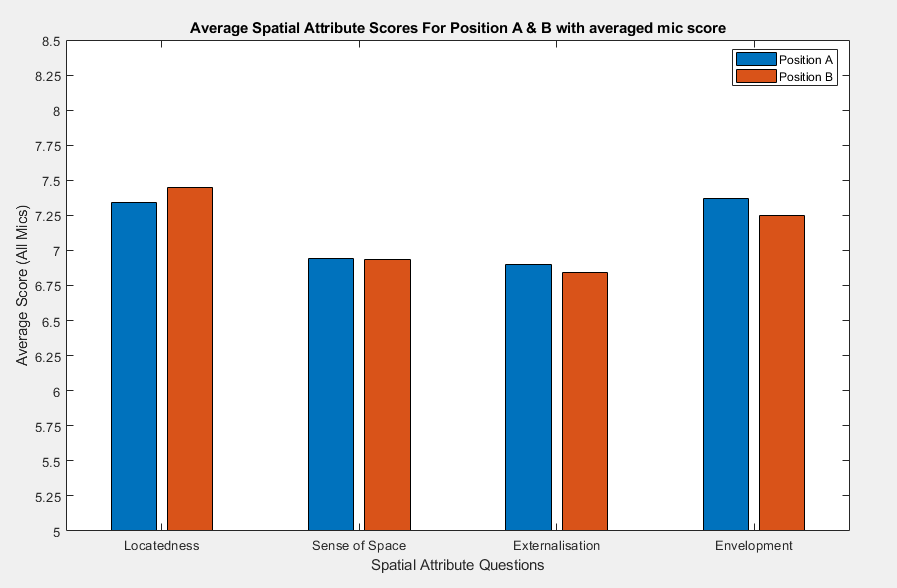
\includegraphics[width=0.5\textwidth]{images/plots/AvB_Bar.PNG}
			\caption{Bar chart showing average spatial attribute score for each spatial attribute at viewing position A and B}
			\label{image:AvsB} 
		\end{figure}

		It can be seen that the average spatial attribute score for viewing position A and B for each spatial attribute are close with the difference in overall mean score being 0.02. Running a Two-Sample T-Test between each of the four spatial attribute groups (e.g A vs B for locatedness etc) indicates no statistical significance. Running the same test for the averaged combined spatial attribute score (average of all four spatial attribute scores) also indicates no statistical significant between viewing position. This is made clear in figure \ref{image:AvsB_dist} illustrating the overall similarity in the distribution of scores for viewing position A and B. \\
		
		% NOTE: Should I display the distributiong as 'normal' or 'kernel'?
		\begin{figure}
			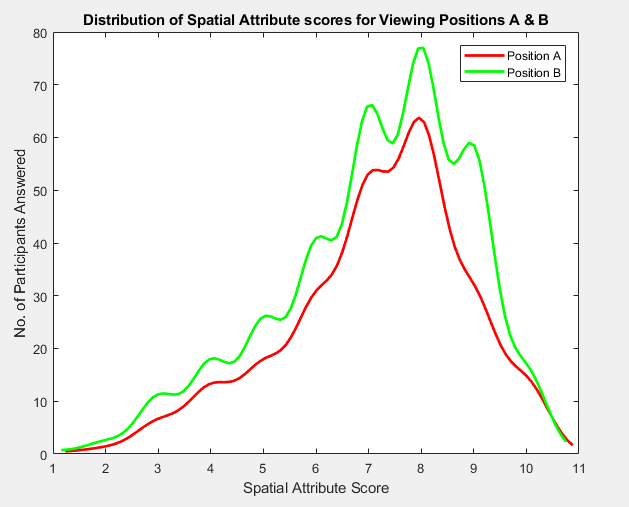
\includegraphics[width=0.5\textwidth]{images/stats/AvsB_sa_stack_all.PNG}
			\caption{Histogram showing the distribution of spatial attribute scores for viewing position A and B. This indicates that viewing position has little effect on spatial qualities in a VR environment.}
			\label{image:AvsB_dist} 
		\end{figure}

		\textbf{Conclusion}\\

		The bar chart indicates that the average SA score are extremely close for each SA with an overall average for both being 7.1. The Two-Sample T-Test indicates that the probability of these results recurring is not unlikely ($p > \alpha (0.05)$) and therefore the results shown are not statistically significant.


	\subsection{Analysis 2: Does the choice of microphone array effect Spatial Attribute score?}
	\label{ana2}

		Breaking down the data showing in figure~\ref{image:AvsB}, figure~\ref{image:sa_allmics} shows the average spatial attribute score across all used microphone configurations. The Anderson-Darling test was used to determine that not all of the sample data (participants scores per microphone) is normally distributed. Due to non-normally distributed data the Kurskal-Wallis (K-W) ANOVA was used to determine whether any of the samples were significantly different. \\

		All groups returned a p-value greater than 0.05 other than 'Sense of Space' which returned a p-value of $p = 0.0227 $. As determined in section~\ref{ana1} there is no statistical significant difference between the data from viewing positions A and B. Therefore the data was separated according to their viewing positions and another K-W test was conducted on each group. This indicated a significant difference within the group of data from viewing position B, returning a p-value $ p = 0.0035 $.

		Using MATLABs \textit{multcompare} function, a post-hoc test was conducted to determine that the sample data for two microphone arrays, OCT and Hamasaki Cube were significantly different to the sample data for the spot microphones, circled in red and blue respectively in figure~\ref{image:sa_allmics}. \\

		% NOTE: SHOULD BE PARAGRAPH BE HERE AS IT HAS BEEN SHOWN THAT THERE IS NO STATISTICAL SIGNIFICANCE IN THE DIFFERENCES IN SCORE?
		Though little statistical significance was found between the difference microphone arrays, by analysing figure~\ref{image:sa_allmics} we can determine which microphones are overall the best choice. The two microphone arrays that showed statistical significance, the OCT and Hamasaki Cube also happen to consistently be among the top scoring microphone arrays across all spatial attributes.

		\textbf{Conclusion} \\

		For most spatial attributes, differences in mic choice is not statistically significant. However when it comes to sense of space, mixing in the microphone arrays, particularly the OCT and Hamasaki cube make a significant difference to listening to just the spot mics on their own.

		\begin{figure}
			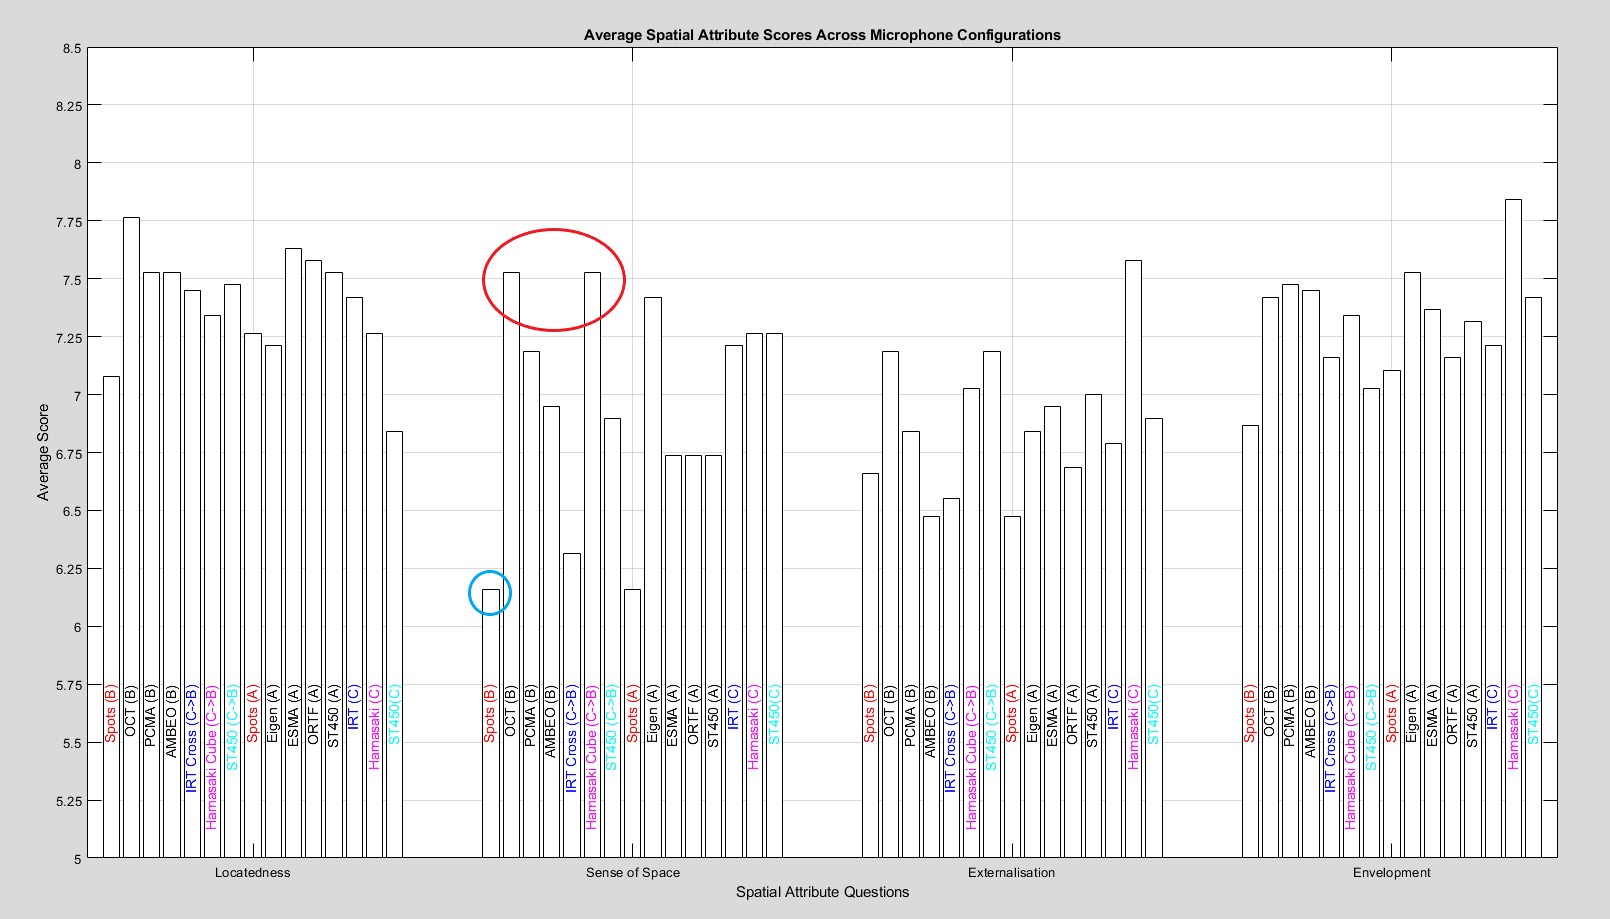
\includegraphics[width=0.5\textwidth]{images/plots/allMics_edit.PNG}
			\caption{Bar chart of the average SA score across all microphone configurations where (X) indicates the microphone location. The microphone names are displayed on their corresponding bar chart where (C->B) indicates a microphone from position C whilst viewing from B and (C) indicates a microphone from position C whilst viewing from position A}
			\label{image:sa_allmics} 
		\end{figure}


	\subsection{Analysis 3: What is the effect of using Directional or Diffuse-Field Arrays?}
	\label{ana3}

		Section~\ref{ana2} revealed no significant difference between using any of the different microphone arrays apart from when it comes to a 'Sense of Space'. However the difference was only found between using just the spot mic mix against mixing the spot mics with either the OCT array or the Hamasaki Cube. As both of these microphone arrays are different from each other, one was used as a directional array and the other as a diffuse field array, and that they were not significantly different from each other, it can also be stated that the use of directional or diffuse field arrays is also not statistically significant.


		Analysing the bar chart in figure~\ref{image:sa_allmics} however it is possible to come to some conclusions about particular microphone configurations. For example, looking at the scores for Sense of Space, the three diffuse field microphone in position C whilst viewing from position A can be said to objectively perform worse than the three of the directional microphones at position A (ESMA, ORTF, ST450). However as the Eigenmke scores higher than all of them, drawing a conclusion that one microphone type is superior would be a incorrect.

		It can also be seen that the OCT scores are always the highest other than for envelopment, where it comes as a close third.

		Analysing the bar chart in figure~\ref{image:sa_allmics} however it is possible to come to some conclusions about particular microphone configurations. For example, looking at the scores for Sense of Space, the three diffuse field microphone in position C whilst viewing from position A all score relatively similar, an average of 7.2 and three of the directional microphones at position A (ESMA, ORTF, ST450) all score the same average score of 6.7. However it is the Eigenmike that levels the difference between these two groups, with an overall higher average higher score. 




	\subsection{Analysis 4: Is there a in perception of timbre with difference viewing positions?}

		
		\begin{figure}
			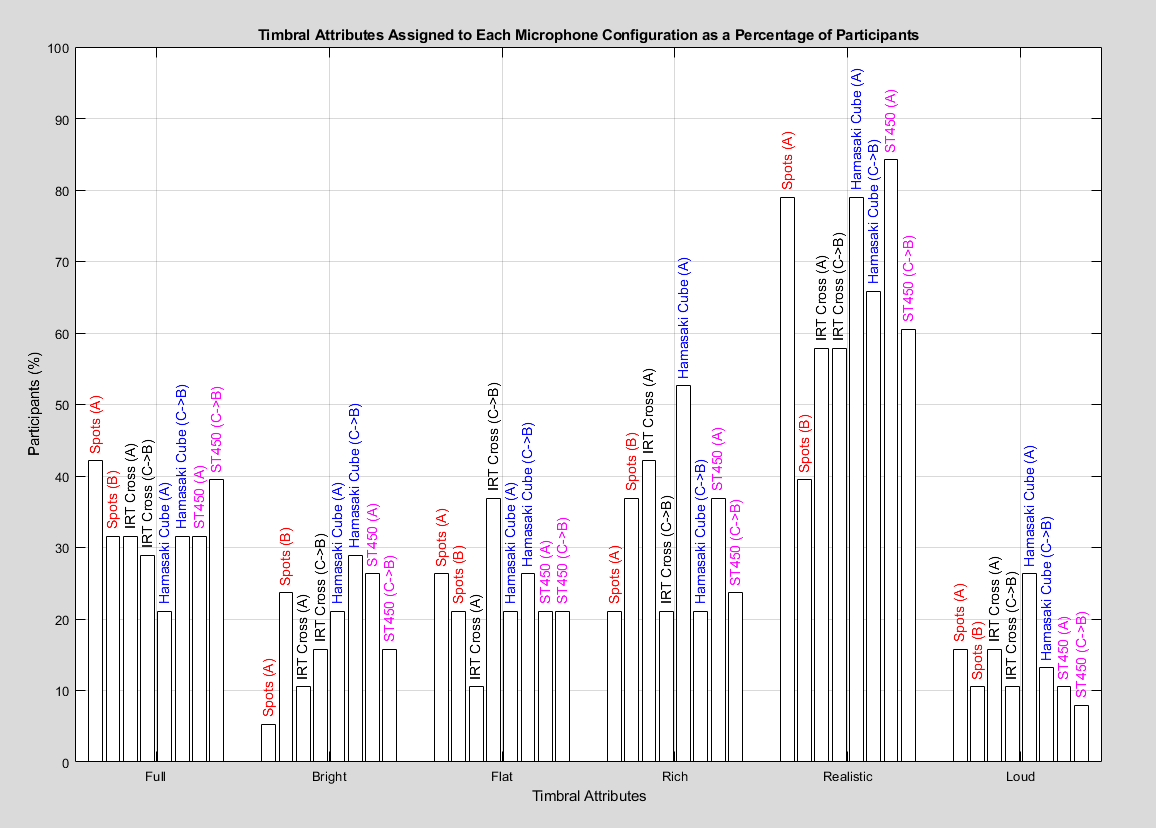
\includegraphics[width=0.5\textwidth]{images/plots/bar_sharedMics.PNG}
			\caption{Bar chart showing the timbral attributes chosen for each microphone array shared between viewing position A and B as a percentage of participants}
			\label{image:ta_sharedmics} 
		\end{figure}		


	\subsection{Analysis 5: Is there a correlation between SA score and selected timbral attributes?}



		\begin{figure}
			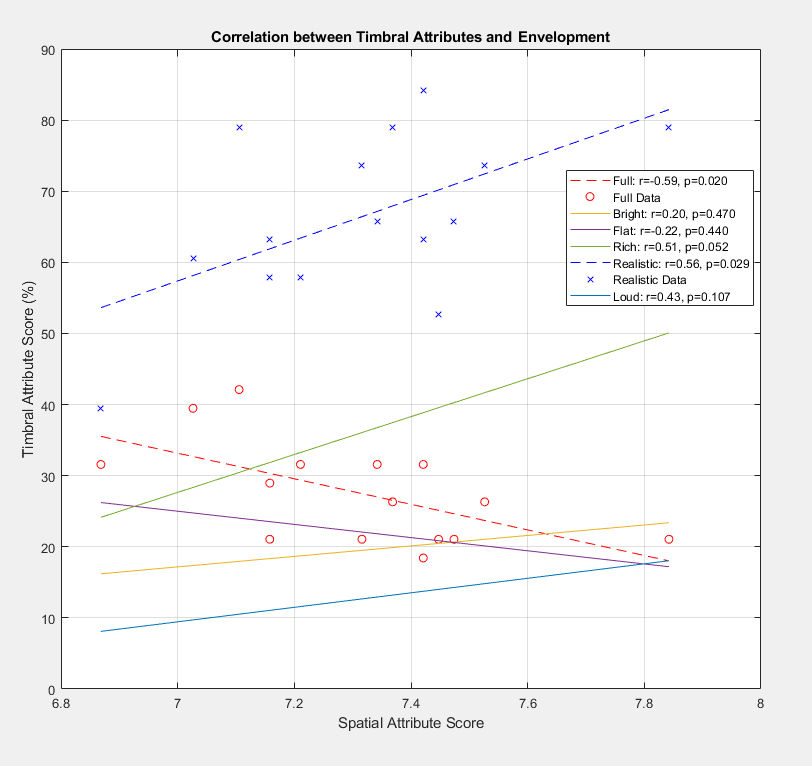
\includegraphics[width=0.5\textwidth]{images/plots/sa_ta_corr_env.PNG}
			\caption{Graph showing correlations between Timbral Attribute and Envelopment scores where dashed lines indicate a statistically significant correlation for which their individual data points have also been plotted.}
			\label{image:corr_env} 
		\end{figure}		
